\section{Instruction set}
The goal of this assignment was to implement a simple multi-cycle MIPS processor in VHDL.
There was a minimal instruction set required to complete this assignment which was implemented in \emph{processor.vhd}:
\begin{itemize}
    \item Several ALU instructions (all working on two registers and storing the result in a third):
        \begin{itemize}
            \item ADD - Addition
            \item SUB - Subtraction
            \item SLT - Store 1 in destination if the first source register is less than second
            \item AND - Bitwise and
            \item OR  - Logical or
        \end{itemize}
    \item BEQ - branch if registers are equal
    \item LW - Load word from memory
    \item SW - Store word to memory
    \item LUI - Store immediate value shifted left 16 bits in a register
    \item J - Jump
\end{itemize}

\section{Architecture}
\begin{figure}[ht]
    \centering
    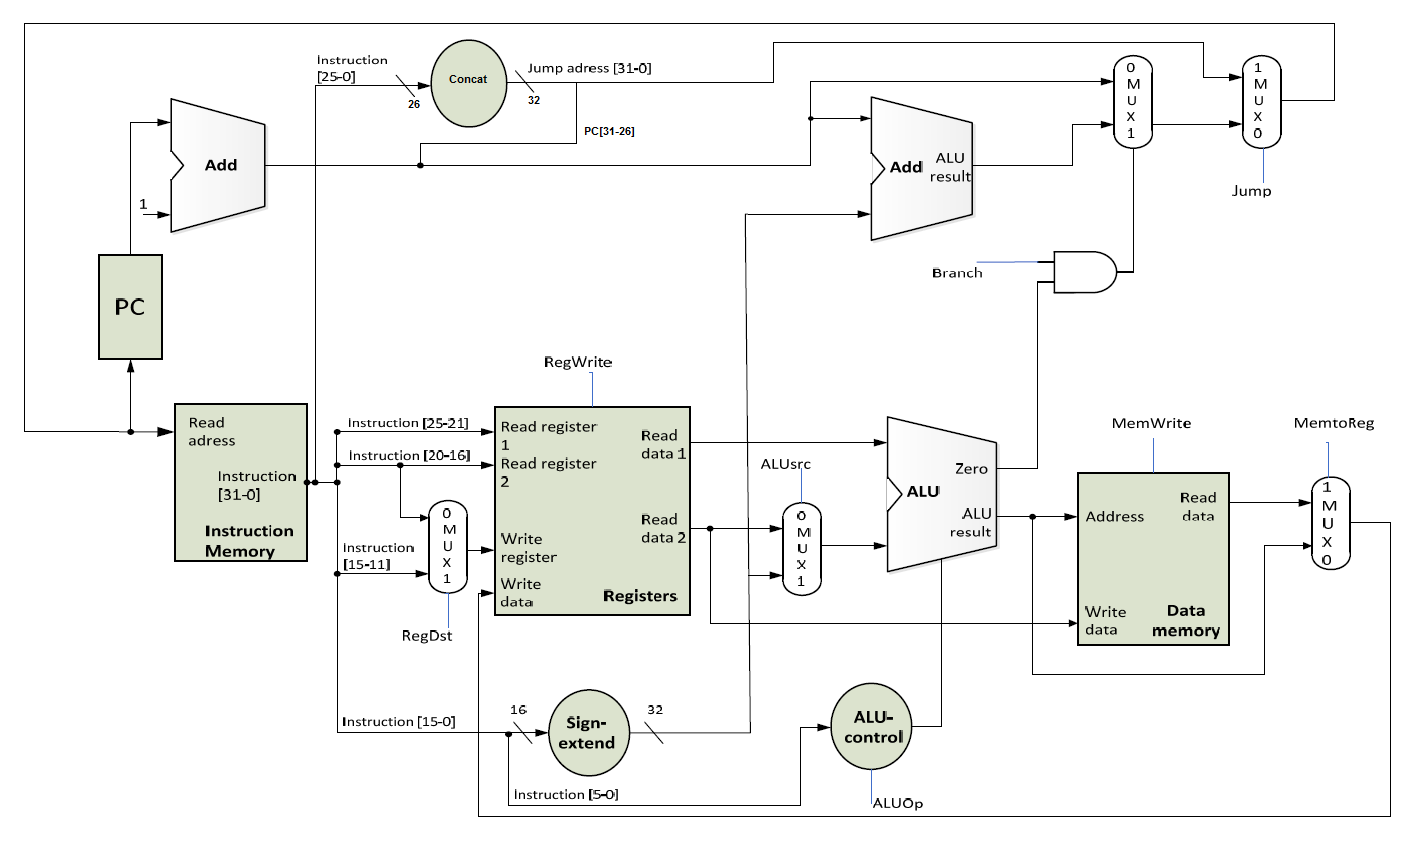
\includegraphics[scale=0.3]{figures/cpu.png}
    \caption{\label{fig:cpuArchitecture}The implemented CPU architecture. Note that the only difference from the architecture suggested in the lecture slides is that the setting of the program counter is moved slightly.} %TODO: reference, page 115 compendium
\end{figure}

The suggested CPU architecture remained mostly unchanged.
The main difference is that instead of retrieving the instruction address from the program counter, it is retrieved directly from the same bus that is used to set the program counter.

\subsection{The control unit}
\begin{figure}[ht]
    \centering
    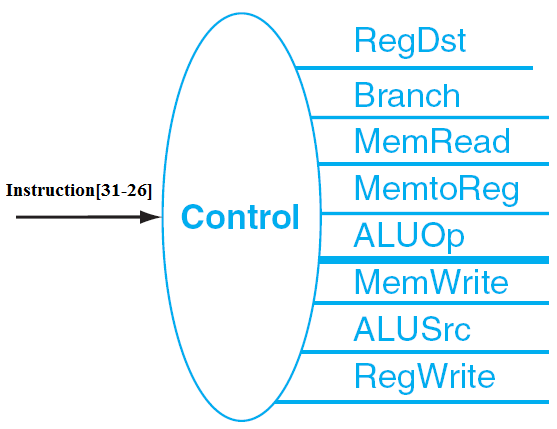
\includegraphics[scale=1.0]{figures/controlunit.png}
    \caption{\label{fig:controlUnit}The control unit.}
\end{figure}
